\documentclass[12pt,a4paper]{article}
\usepackage[utf8]{inputenc}
\usepackage[german]{babel}
\usepackage[T1]{fontenc}
\usepackage{amsmath}
\usepackage{amsfonts}
\usepackage{amssymb}
\usepackage{graphicx}
\usepackage[left=2.5cm,right=2.5cm,top=2cm,bottom=2cm]{geometry}
\usepackage{float}
\author{Gruppe C14 \\ Julián Häck, Martin Koytek, Lars Wenning, Erik Zimmermann}
\begin{document}
\section{z.B. Widerstand, Teilversuch 4.1}
\subsection{Versuchsbeschreibung}
%Kurze Darstellung der physikalischen Grundlagen und Ziele der Versuche, %die zum Verständnis
%des Versuches/Protokolls benötigt werden. (max. 1 Seite)
Wir betrachten zunächst ein mathematisches Pendel welches wir später durch die Verschiebung des Pendelkörpers ergänzen um das physikalische Pendel betrachten zu können.
Die Bewegungsgleichung zum mathematischen Pendel nach der Kleinwinkelnäherung lautet:
\begin{equation*}
J \cdot \ddot{\phi} = -m_s \cdot g \cdot l \cdot \phi 
\end{equation*}
Mit $m_T=m_S$ und Lösen der daraus folgenden DGL ergibt sich die allgemeine Lösung einer harmonischen Schwingung:
\begin{equation*}
\phi(t)=A\cdot cos(\omega t) + B \cdot sin(\omega t)
\end{equation*}
Nun gleichen wir unser $\omega$ der Pendelstange mit dem $\omega$ der Pendelstande mit Pendelkörper, durch verschieben des Pendelkörpers an der Pendelstange, an:
\begin{equation*}
\frac{D_p}{J_p}=\frac{D_st}{J_st}:=\omega_st^2=\omega^2=\omega_p^2
\end{equation*}
Nun können wir einen ausgedehnten Pendelkörper betrachten der an einer masselosen Stange befestigt ist.
Aus dem sich daraus ergebenden
\begin{equation*}
\omega^2=\frac{m_p \cdot g \cdot l_p}{\frac{1}{2}m_p r_p^2+m_pl_p^2}
\end{equation*}
lässt sich nun
\begin{equation*}
g=\omega^2 l_p (1+\frac{r_p^2}{2 l_p^2})
\end{equation*} 
berechnen.
\newpage
\subsection{Versuchsaufbau und Durchführung}
%Genaue Beschreibung der verwendeten Aufbauten unter Verwendung von Skizzen oder Photos
%Beschreibung der Messwerterfassungseinstellungen (eingestellte Messzeiten, Messbedingungen,
%Trigger, Anzahl der Messungen) und der Durchführung der Versuche. (max. 1 Seite)
\begin{figure}[H]
\centering
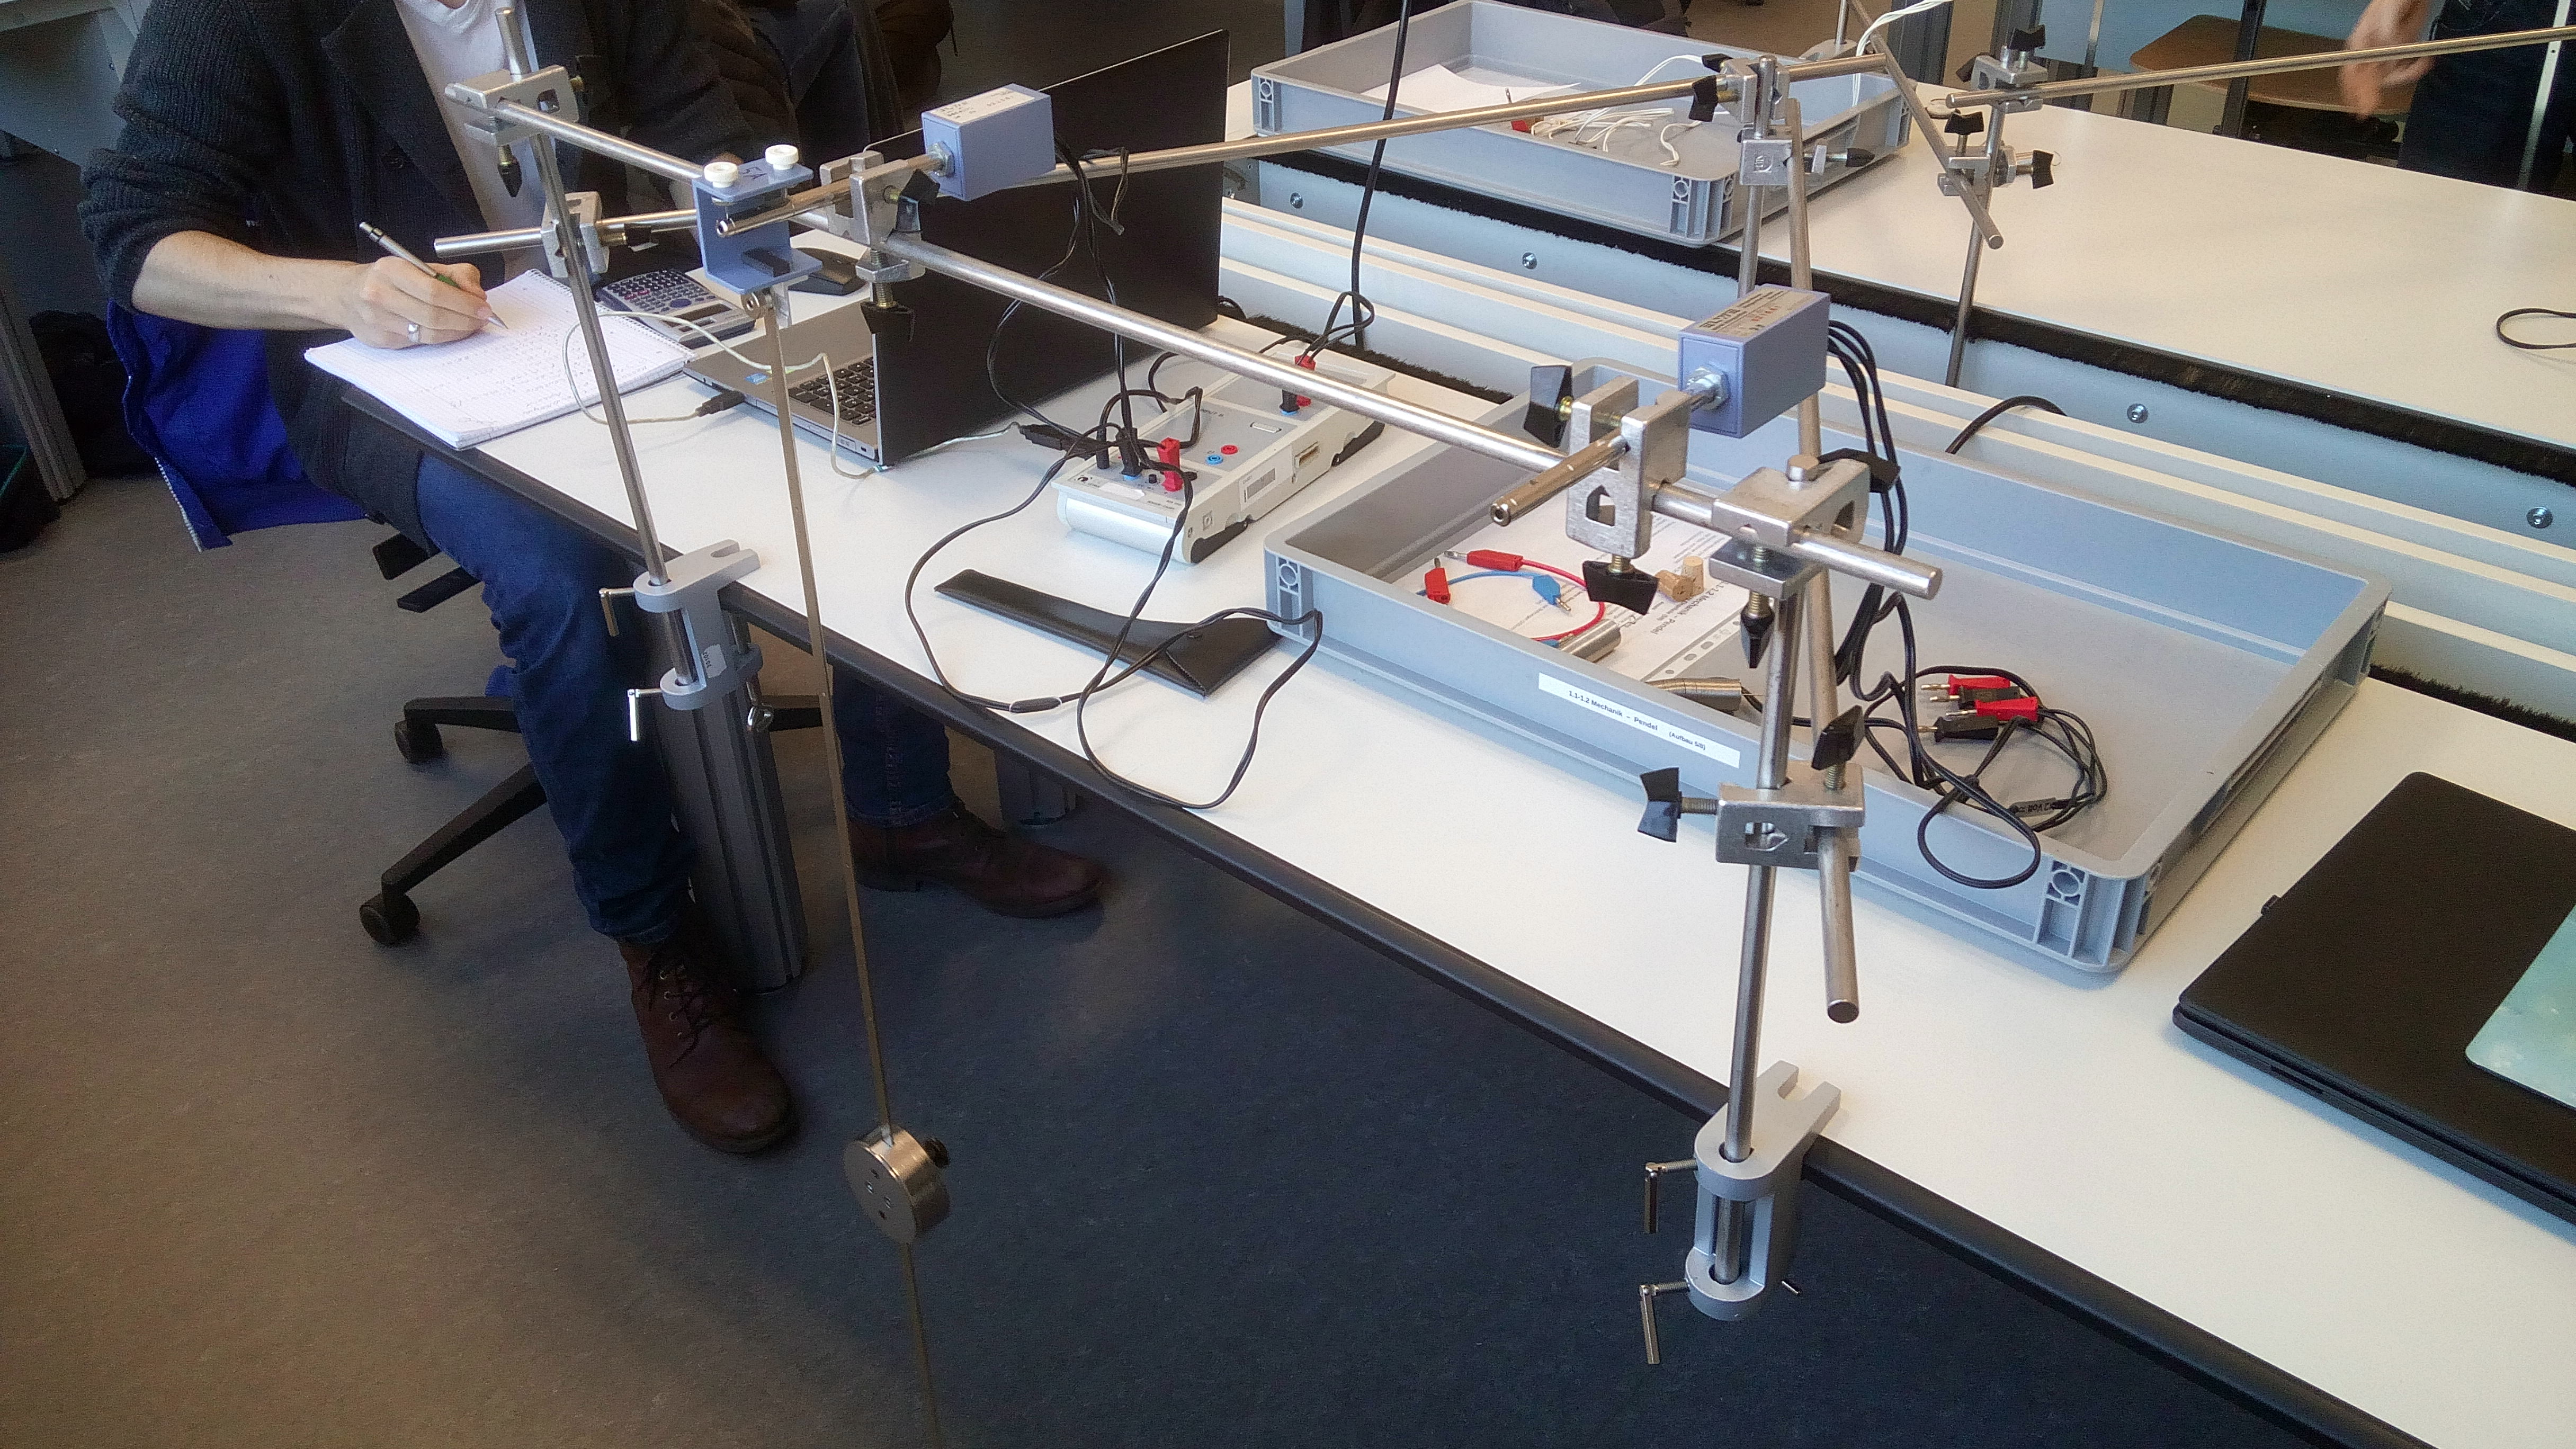
\includegraphics[scale=0.1]{Bilder/Einzelpendel.jpg}
\caption{Versuchsaufbau mit Pendelkörper}
\end{figure}
Unser Versuchsaufbau besteht aus einem Dreibein um die Stabilität zu erhöhen, an dem dann der Winkelabnehmer befestigt wurde. In die Nut des Winkelabnehmer wurde dann die Aufhängung des Pendels aufgelegt.
Nun wurde zunächst die Pendelstange ohne Pendelkörper in Schwingung versetzt und die Hallspannung des Winkelabnehmers aufgezeichnet und die Frequenz per FFT bestimmt.
Anschließend wurde der Pendelkörper angebracht, das Pendel erneut ausgelenkt und die Schwingung aufgezeichnet. Dies wurde wiederholt bis die Frequenz mit der der Pendelstange ohne Pendelkörper übereinstimmte.
Dieser Aufbau wurde nun vier mal in Schwingung versetzt und die Hallspannungen aufgezeichnet.
Zum Schluss wurde dann die Länge des Pendels, der Abstand des Pendelkörpers zum Aufhängepunkt und der Radius des Pendelkörper gemessen.
\newpage
\subsection{Versuchsauswertung}

\subsubsection{Rohdaten}
1 Seite
\subsubsection{Transformation der Rohdaten}
Transformation der Rohdaten und Modellanpassung. (1 Seite)
\subsubsection{Analyse}
Analyse der Daten inklusive Fehlerrechnung Residuen und Pullverteilung. (1 Seite)
\subsubsection{Fazit}
Diskussion der Ergebnisse und Vergleich der erzielten Ergebnisse mit theoretischen Vorhersagen.
(1 Seite)

\end{document}